\chapter{Bipolar}
\label{applications-prior_level_vals}

The meta-analysis of data from a systematic review on the descriptive epidemiology of bipolar disorder provides an excellent example of the effects of informative priors on levels of age-specific incidence and remission hazards.

Bipolar disorder is a mental disorder that causes mood swings fluctuating between euphoric highs called manic episodes and depressive lows, interspersed by periods of residual symptoms.  Manic episodes may last from days to months, causing personal, social and work-related problems.  Mood swings may occur as infrequently as yearly or as frequently as several times a day.  Extreme behavior changes accompany mood changes, and it is not uncommon for sleeping, eating or activity patterns to change with manic and depression episodes.  There is no clear cause for episodes, but life changes, medications and sleeplessness may trigger manic periods.  While there is no cure, treatment helps manage mood swings and related symptoms \cite{american_diagnostic_2000, national_bipolar_2012, national_bipolar_2011, mayo_bipolar_2012}.

The disease modeling of bipolar disorder was based on literature describing it as a chronic illness with little or no complete remission. This approach differed to the modeling of chronic episodic mood disorders like major depressive disorder where an estimate of disease duration rather than remission is required \cite{american_diagnostic_2000}.

Thirty-two studies were identified for prevalence, covering 22 countries in 11 GBD world regions (\ref{tab:bipolar_data}). Two studies were identified for incidence, both from the United States of America. Seven studies were identified for excess mortality, from 5 high income countries. We found no studies reporting on complete remission (equivalent to cure rather than a temporary reduction in symptom levels as clinicians tend to define 'remission') from bipolar disorder as defined by GBD, consistent with the description in the literature that there is no cure for bipolar disorder.

\begin{table}[h]
    \begin{center}
        \caption{ Frequency of bipolar data types by region used in estimating disease parameters}
        \label{tab:bipolar_data}
        \begin{tabular}{|l|c|c|c|c|}
            \hline
                Region & Prevalence & Incidence & Remission & Mortality \\
            \hline
                Europe, Western & 24 & 0 & 0 & 13 \\
                North America, High Income & 19 & 2 & 0 & 4 \\
                Australasia & 16 & 0 & 0 & 0 \\
                Asia, East & 12 & 0 & 0 & 0 \\
                Asia Pacific, High Income & 8 & 0 & 0 & 2 \\
                Latin America, Tropical & 4 & 0 & 0 & 0 \\
                Sub-Saharan Africa, East & 2 & 0 & 0 & 0 \\
                North Africa/Middle East & 2 & 0 & 0 & 0 \\
                Latin America, Southern & 2 & 0 & 0 & 0 \\
                Latin America, Central & 2 & 0 & 0 & 0 \\
                Europe, Eastern & 2 & 0 & 0 & 0 \\
                Sub-Saharan Africa, West & 0 & 0 & 0 & 0 \\
                Sub-Saharan Africa, Southern & 0 & 0 & 0 & 0 \\
                Sub-Saharan Africa, Central & 0 & 0 & 0 & 0 \\
                Oceania & 0 & 0 & 0 & 0 \\
                Latin America, Andean & 0 & 0 & 0 & 0 \\
                Europe, Central & 0 & 0 & 0 & 0 \\
                Caribbean & 0 & 0 & 0 & 0 \\
                Asia, Southeast & 0 & 0 & 0 & 0 \\
                Asia, South & 0 & 0 & 0 & 0 \\
                Asia, Central & 0 & 0 & 0 & 0 \\
                Total & 93 & 2 & 0 & 19 \\
            \hline
        \end{tabular}
        \end{center}
    \end{table}

There was considerable variability in the data. For instance, estimates were reported across multiple age groups (specific or broad), they were based on different coverage areas (community or national) and they were either sex specific or for both sex combined. This data has been summarized in greater detail elsewhere {Ferrari, 2011 #1574; Ferrari, 2011 #1581}.

    \begin{figure}[h]
        \begin{center}
            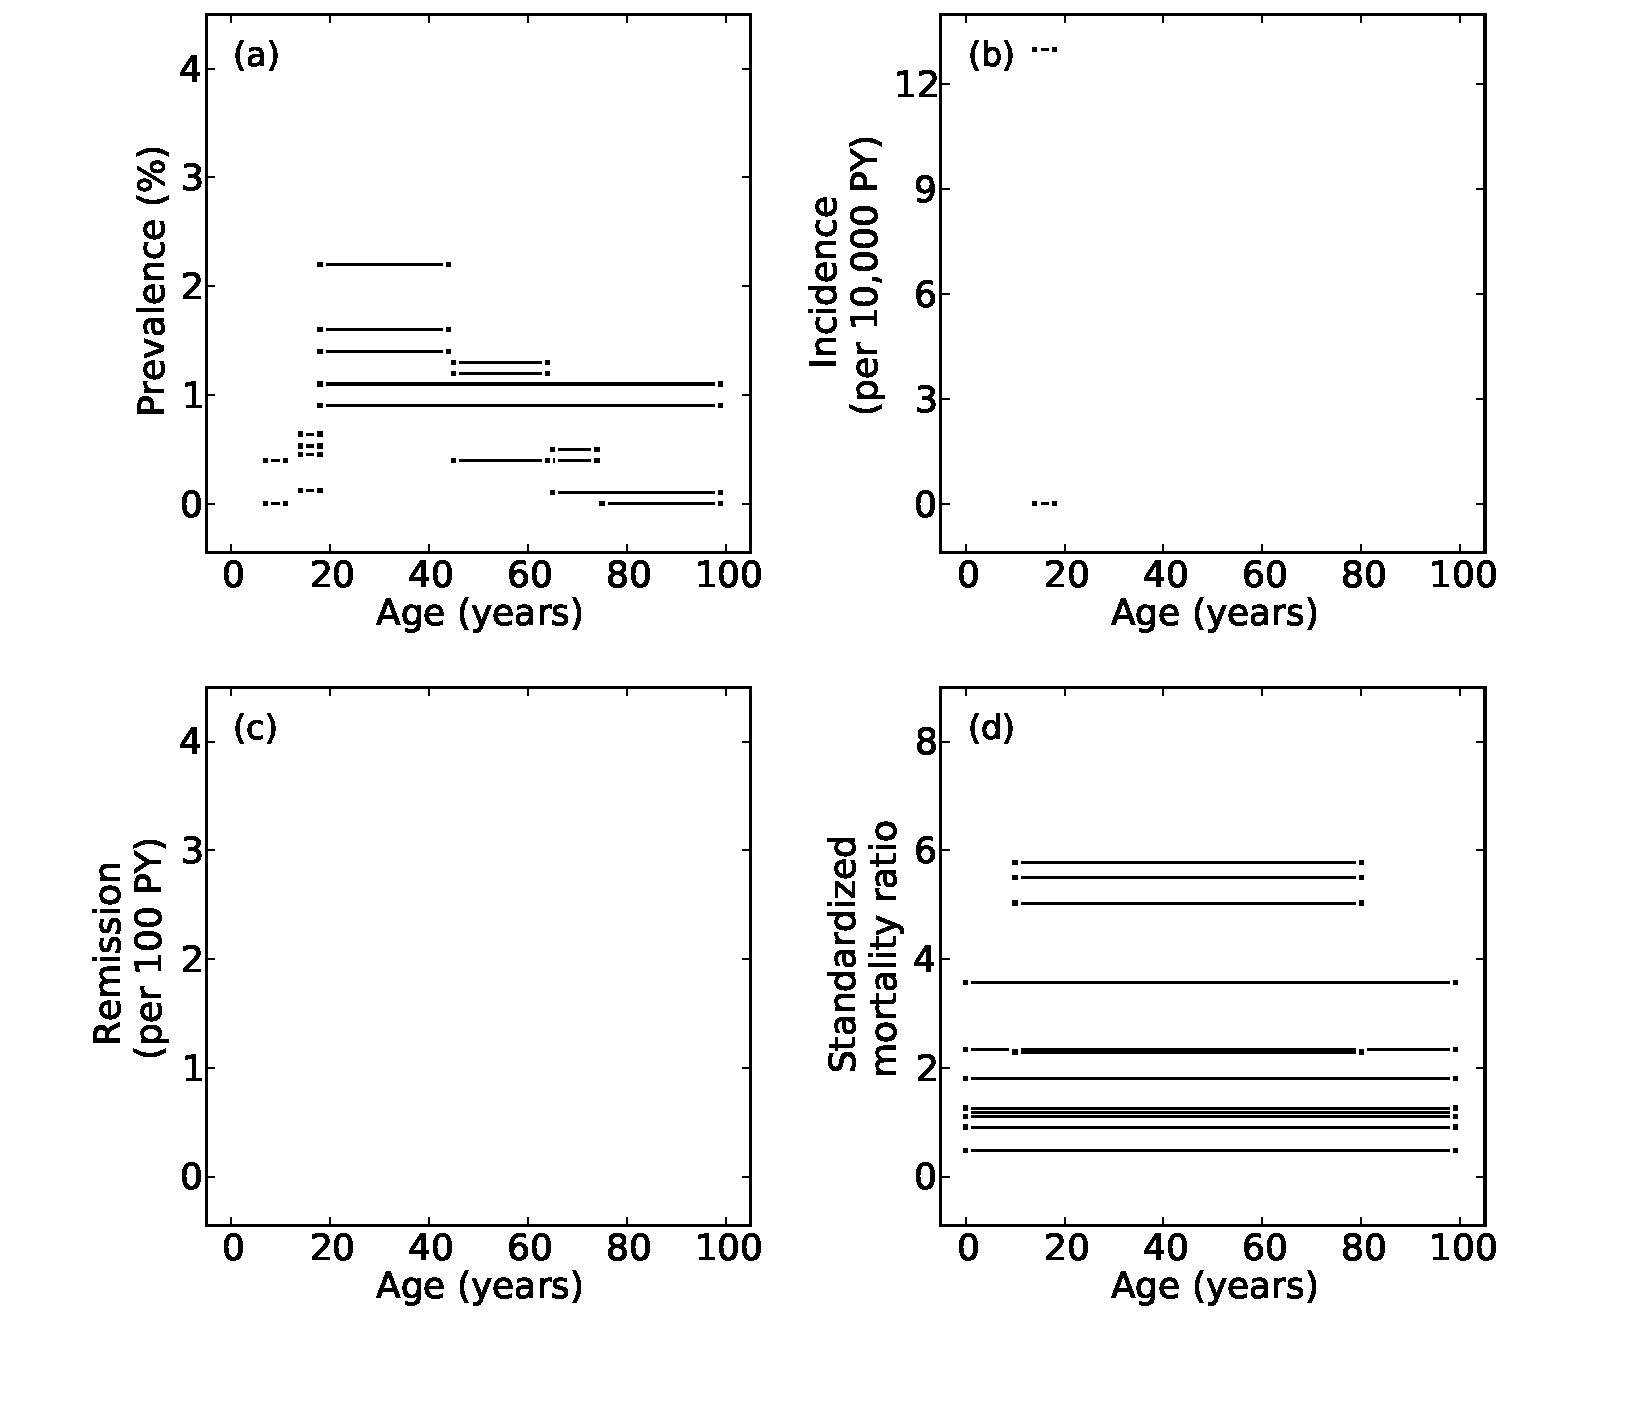
\includegraphics[width=\textwidth]{bipolar-data.pdf}
            \caption{Data included for the modeling of bipolar disorder.  Thirty-two studies were identified for prevalence, covering 22 countries in 11 GBD world regions. No studies reporting on complete remission (equivalent to cure rather than a temporary reduction in symptom levels as clinicians tend to define 'remission') were found.}
            \label{fig:app-bipolar data}
        \end{center}
    \end{figure}

\section{Prevalence and Incidence age of onset}
While there is evidence to suggest that bipolar disorder commonly starts in the mid-teens or early twenties, there is still disagreement over a minimum age of onset {Goodwin, 2008 #208}. Even though symptoms can be tracked back to childhood, setting a threshold for diagnosis is difficult given that current diagnostic criteria are based on adult presentation of the disorder. The literature and expert advice on this issue suggests that although pre-pubertal bipolar disorder is rare, a distinct phenotype can exist. In order to capture as much of the burden attributable to this disorder, a minimum age of onset of 10 years and a maximum of 90 years was set for prevalence and incidence.

    \begin{figure}[h]
        \begin{center}
            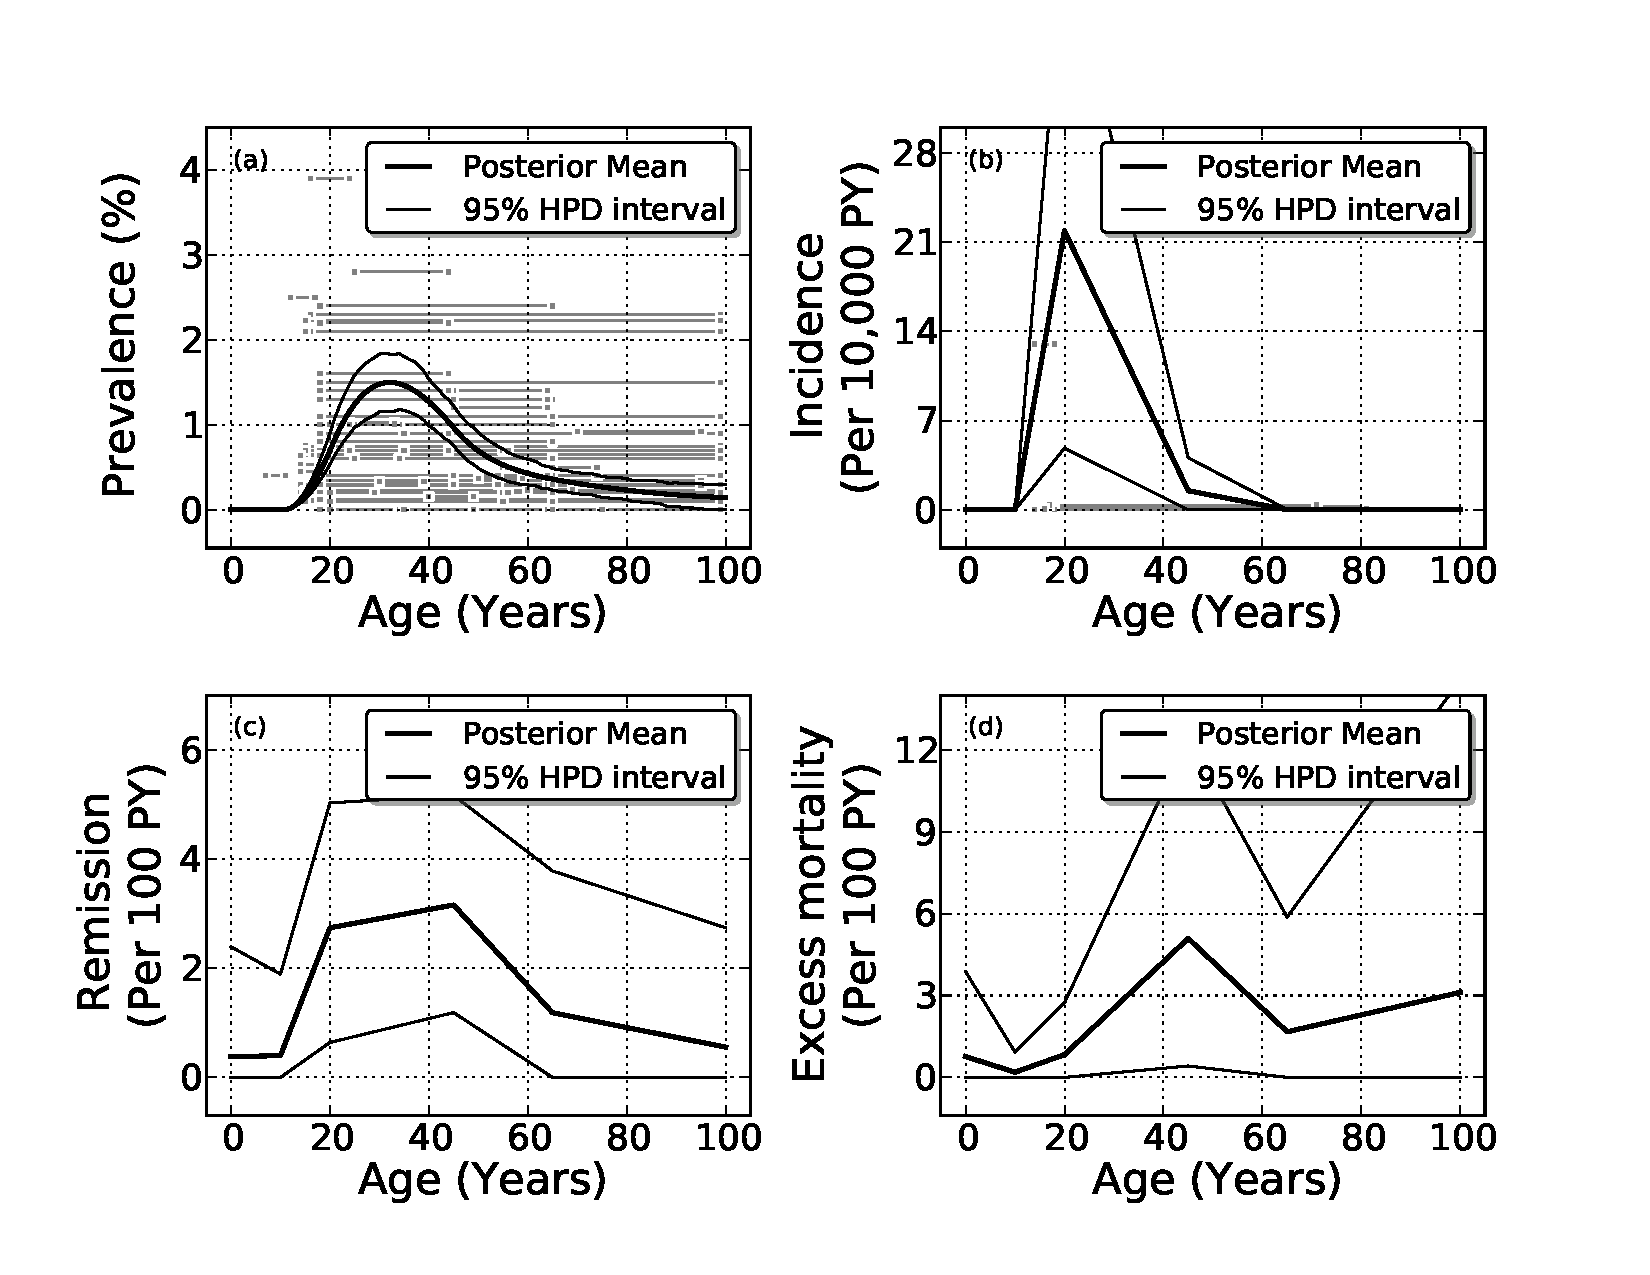
\includegraphics[width=\textwidth]{bipolar-zero_before_ten.pdf}
            \caption{Bipolar epidemiologic parameters for Western Europe males in 1990.  Priors set restrictions of the age of onset so that prevalence and incidence is 0 before age 10 and after age 65.}
            \label{fig:app-bipolar fit}
        \end{center}
    \end{figure}

While expert priors are useful in guiding the modeling process, they may have unintended effects as discussed in Chapter ??(5.2).  Choosing to have no age restrictions on incidence and prevalence, the age-specific burden of disease differs greatly, as shown in figure \ref{fig:app-bipolar bounds}.

    \begin{figure}[h]
        \begin{center}
            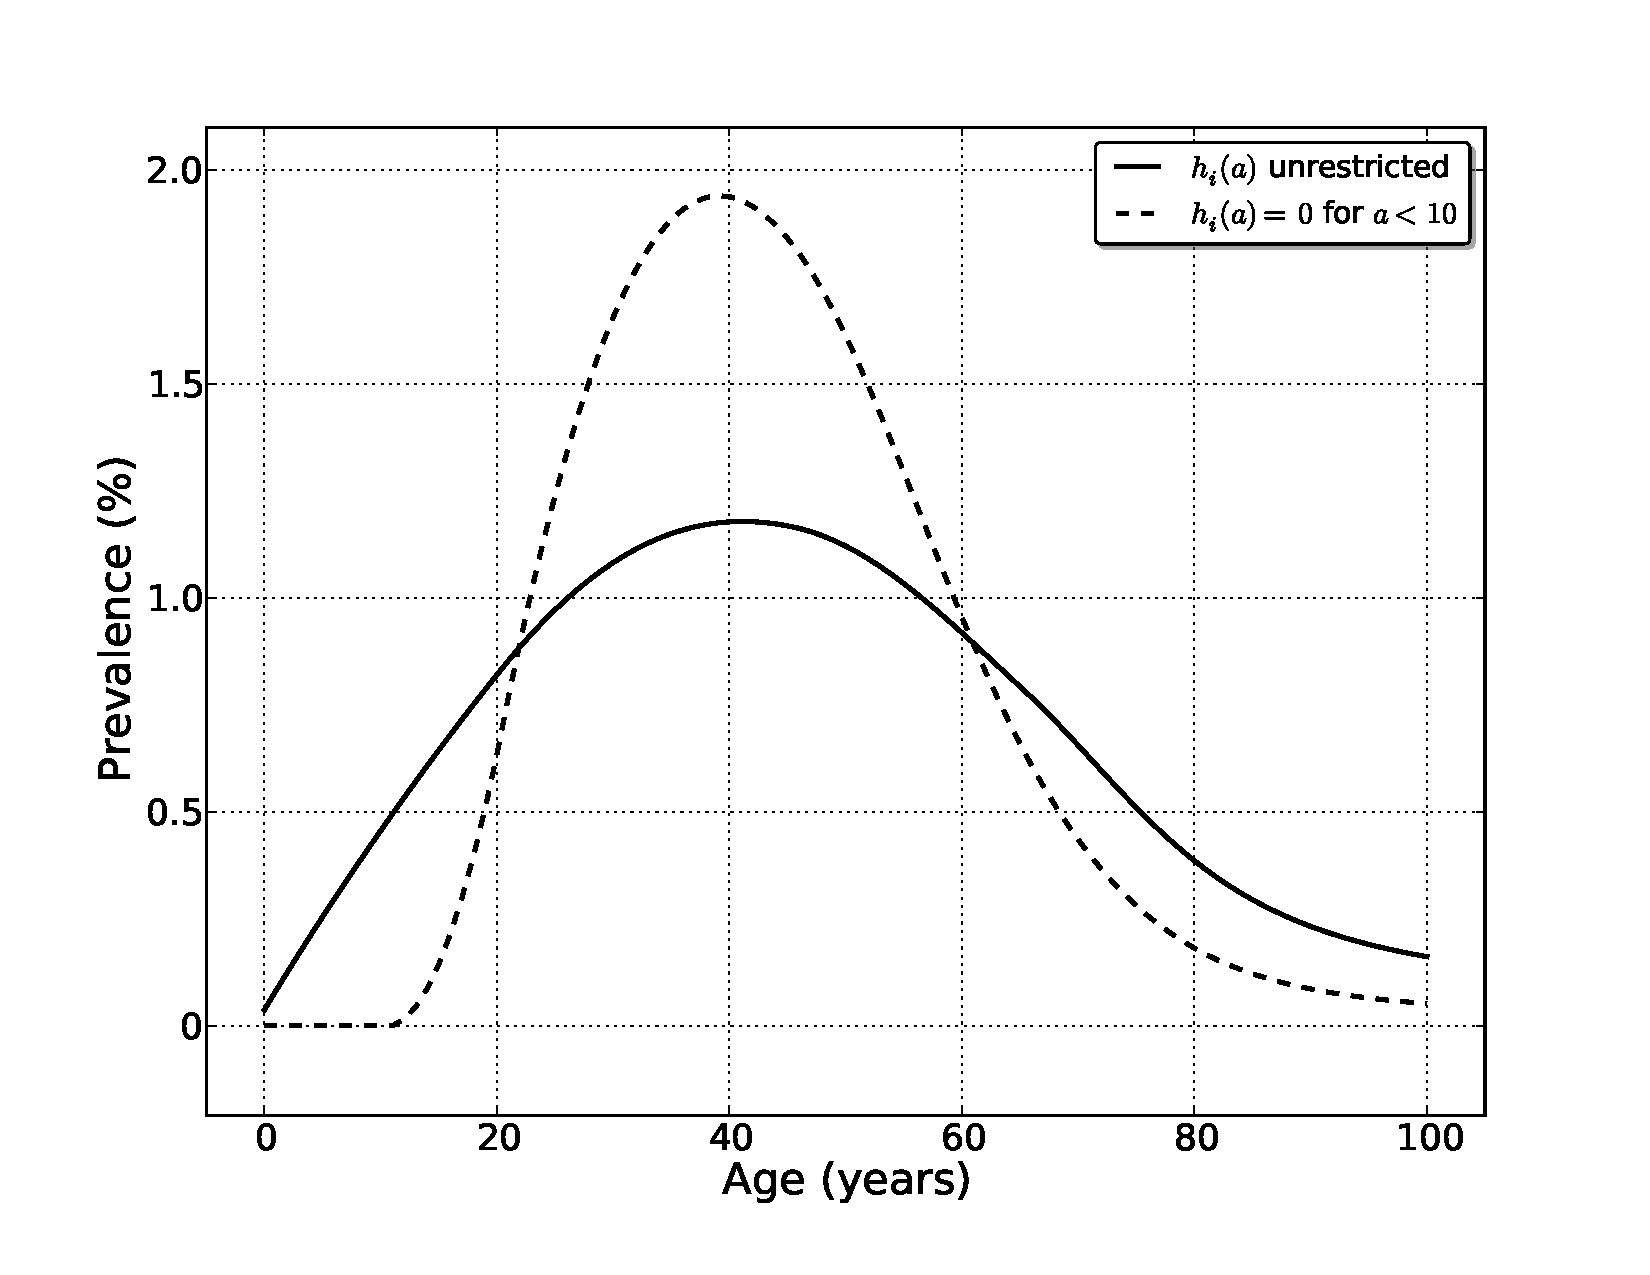
\includegraphics[width=\textwidth]{bipolar-bounds.pdf}
            \caption{The effect of priors can have a large effect on the disease model.  Here, the prevalence of bipolar disorder in Western Europe males in 1990 differs greatly when there priors to set limits on prevalence and incidence to be 0 before age 10 and after age 90.}
            \label{fig:app-bipolar bounds}
        \end{center}
    \end{figure}

Like the age of onset, little is known about the upper age limit of bipolar disorder.  Therefore a prior restricts the upper age limit to 65 years for incidence as it led to the most plausible fit to the data.  Using expert knowledge set plausible bounds on the level of disease is useful in modeling noisy data, but changes the upper age limit produce unexpected changes as shown in figure \ref{fig:app-bipolar onset}.

    \begin{figure}[h]
        \begin{center}
            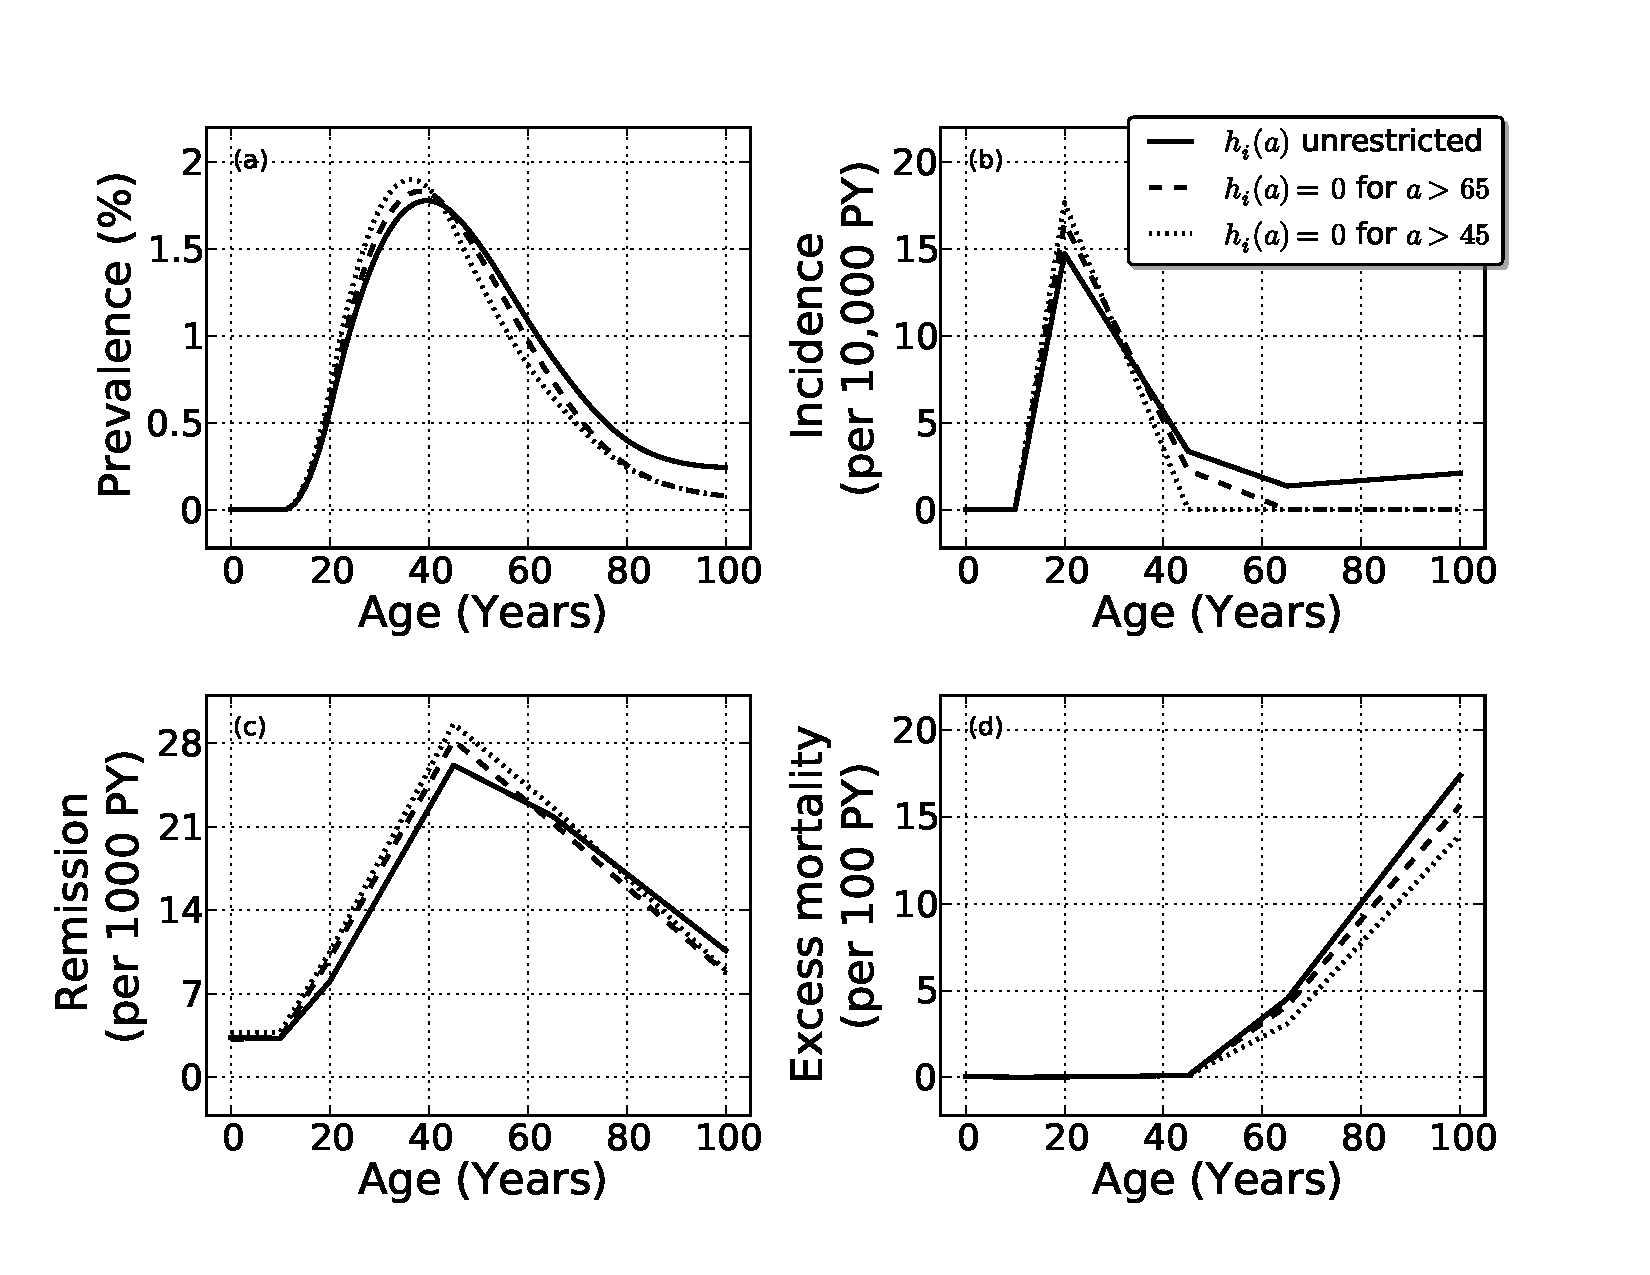
\includegraphics[width=\textwidth]{bipolar-45_65_100.pdf}
            \caption{Estimated prevalence, incidence, remission and excess mortality for Western Europe males with bipolar disorder in 1990.  Priors that restrict the upper age limit of incidence to 45, 65 and 100 propagate through the model to changes in remission and excess mortality.}
            \label{fig:app-bipolar onset}
        \end{center}
    \end{figure}

\section{Residual v Remission}
Although residual symptoms can be less severe than manic and depressive episodes, they still lead to some disability and therefore burden.  However since an average episode of bipolar disorder is believed to last for about 3 months or more {Angst, 2000 #196;Goodwin, 2008 #208}, estimates of point prevalence assessing symptoms within the past month or less, will likely miss cases of bipolar disorder in a residual episode and underestimate prevalence.

The terms 'residual' and 'remission' have very different implications for GBD.  A residual state involves mild symptoms with mild disability which still contribute to burden. Remission is equivalent to cure rather than a temporary reduction in symptom levels hence does not contribute to burden. Since there is no consistent use of these terms in the bipolar literature, we were unable to include any remission data in the bipolar modeling. Instead, expert guidance was sought to set an upper bound on remission hazard of 5 per 100 person-years, yielding a plausible fit to the existing data. To understand the sensitivity of model estimates to this assumption, we also considered upper bounds on remission hazard of 0 and 10 per 100 person-years.  As shown in the figure \ref{fig:app-bipolar remission}, this leads to large changes in the estimated excess mortality.

    \begin{figure}[h]
        \begin{center}
            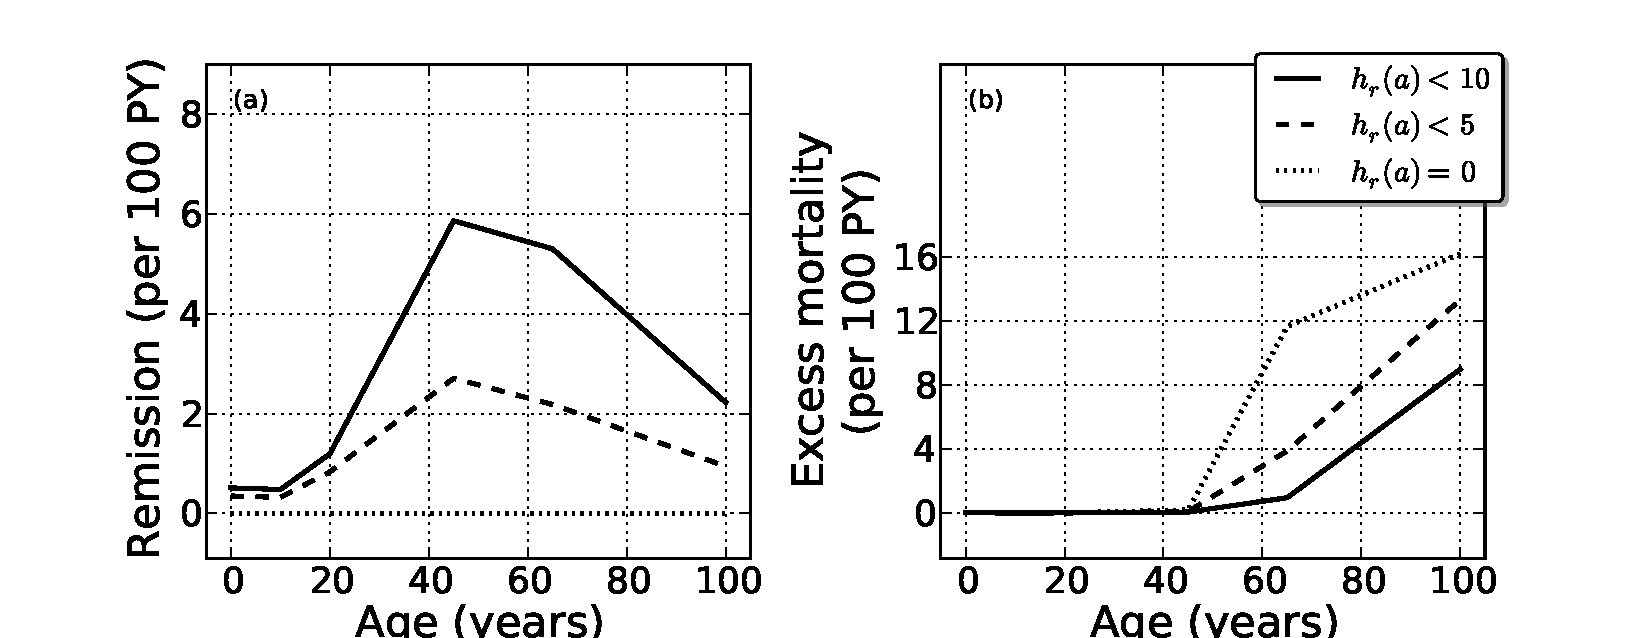
\includegraphics[width=\textwidth]{bipolar-0_5_10.pdf}
            \caption{With no data for bipolar disorder remission, a prior for the level of remission can have unexpected results, as shown above for Western Europe males in 1990.  Changing the remission prior levels to 0.0, 0.05 or 0.1 (units?) for bipolar disorder also changes the excess mortality.}
            \label{fig:app-bipolar remission}
        \end{center}
    \end{figure}

